\chapter{Interlude on Bundles}\label{ch:bundles}


Over the last few chapters, we have taken a very concrete picture of vectors and have made it successively more abstract. At this point, physics students are well in their right to ask: where are there vector spaces in physics?\sidenote{This interlude is ``for culture'' and is outside the main narrative of the course.}

\section{Tangent Planes}


Consider the sphere---perhaps this is the surface of the Earth. We are little specks on the surface of the sphere. To be fancy, we call this sphere a \textbf{manifold}\index{manifold}.\sidenote{You can think of this as a possibly curvy space of positions.} To each us, the world appears to be flat.\sidenote{We say that \emph{locally} our space appears to be flat.} We can make a chart of our local \emph{neighborhood} and draw a \emph{map} on a piece of paper where we describe the apparently-flat space around us, see \bigidearef{}~\ref{idea:2d:chart}. We can imagine that this map is a plane that is tangent to the surface of the earth.
% 
\begin{marginfigure}%[th]
    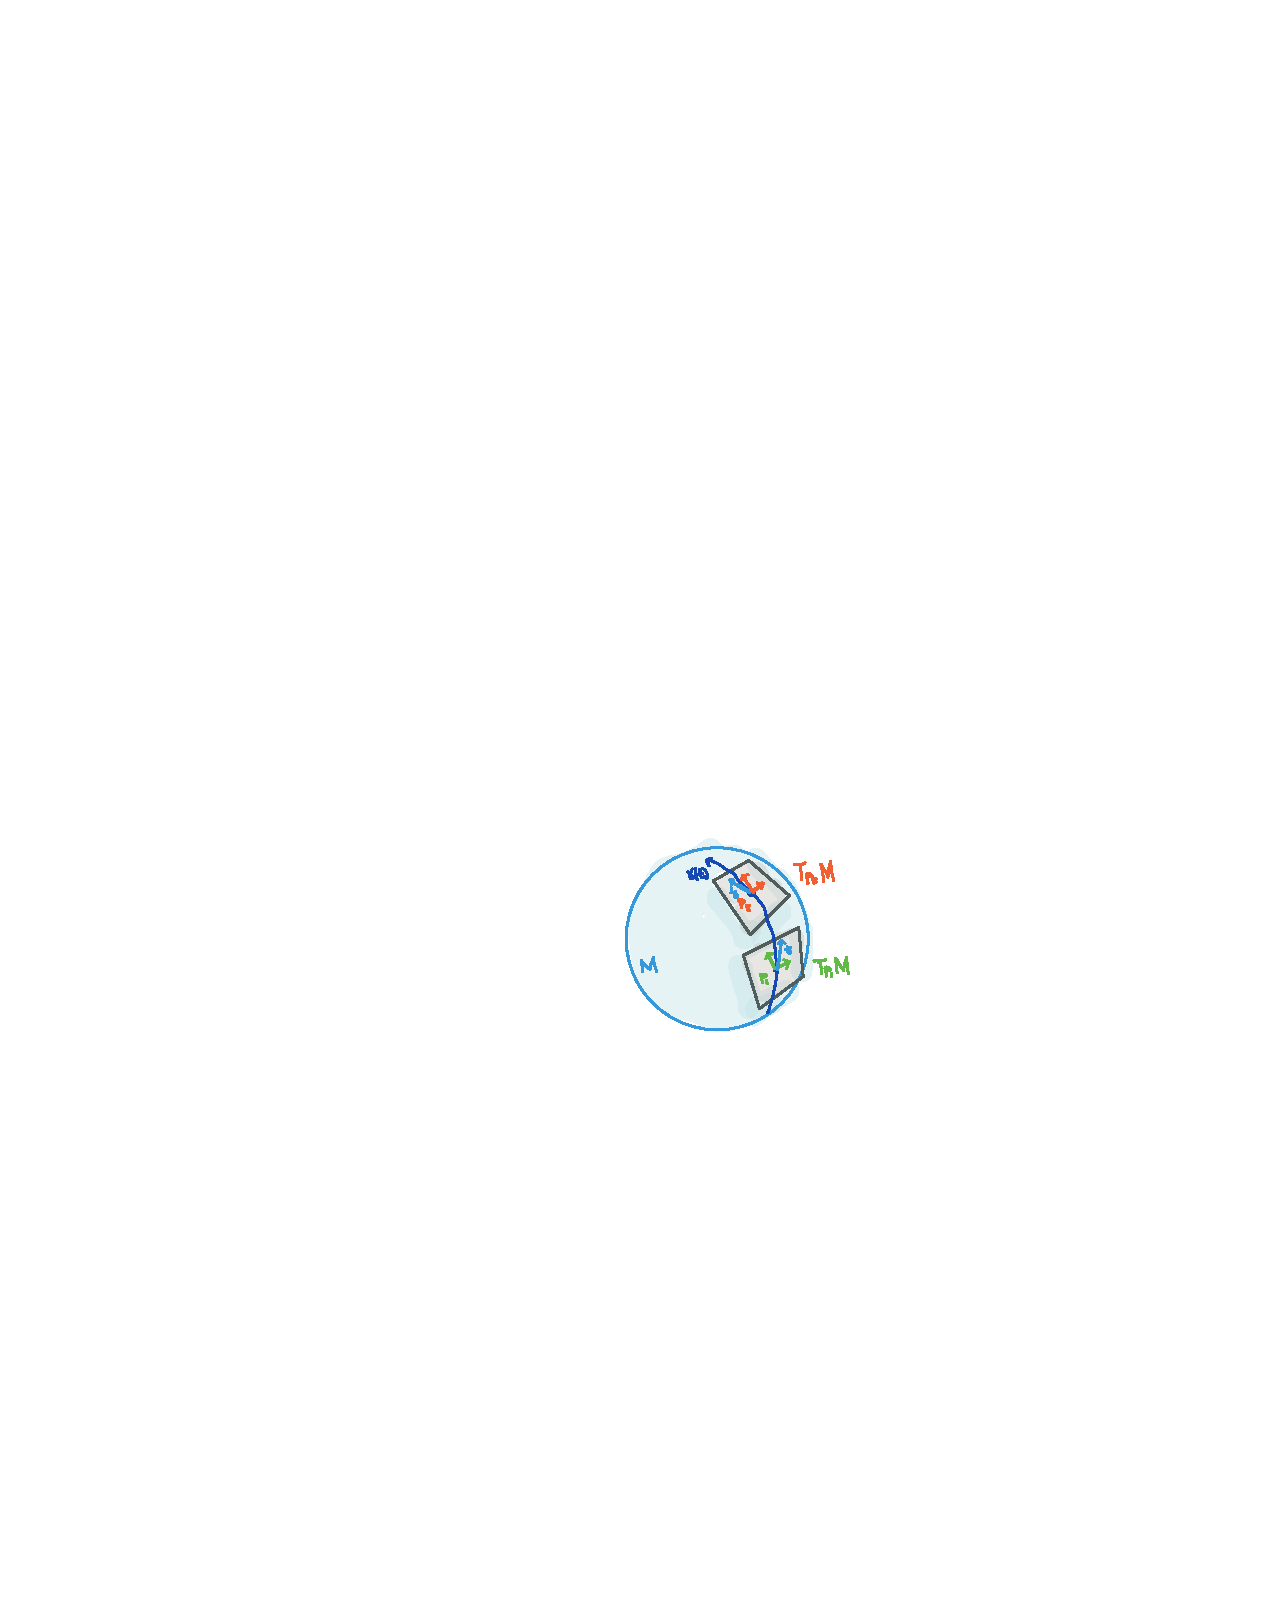
\includegraphics[width=\textwidth]{figures/TangentBundle.pdf}
    \captionsetup{font={scriptsize,sf}}
    \caption{Two tangent planes, $\textnormal{T}_{p_{1,2}M}$ over a manifold $M$. A curve $\gamma(t)$ through the manifold has velocity vectors $\dot{\gamma}(t)$ that live in the tangent planes at each point $\gamma(t)=p_i$.}
    \label{fig:tangent:bundle:sphere}
\end{marginfigure}
% 

If we were somewhere else on the sphere, perhaps in the southern hemisphere, then we would again observe a locally flat space that we could imagine as a tangent plane. Figure~\ref{fig:tangent:bundle:sphere} draws two such tangent planes, perhaps as seen by an observer from far away, like the International Space Station. In the figure, the two tangent planes are called $\textnormal{T}_{p_1}M$ and $\textnormal{T}_{p_2}M$. The key observation in this example is that the tangent planes at different points $p_1$ and $p_2$ are similar, but they have \emph{different orientations}. Viewed from the International Space Station, it is clear that the vectors in $\textnormal{T}_{p_1}M$ live in a totally different vector space than those in $\textnormal{T}_{p_2}M$. From the perspective far away from earth, the vectors on these tangent planes actually have \emph{three} components. Accounting for the third dimension, the \emph{span} of vectors in $\textnormal{T}_{p_1}M$ is different from the span of vectors in $\textnormal{T}_{p_2}M$.


In this figure we have also drawn a path, $\gamma(t)$. You can imagine this as the trajectory of someone journeying from the south pole to the north pole.\sidenote{Like those old \emph{Indiana Jones} cuts between scenes that shows the airplane on the map.} In this notation, $\gamma(t)$ specifies the longitude and latitude of the traveler as a function of time, $t$. The time derivative $\dot\gamma(t)=\D{\gamma}/\D{t}$ is the \emph{velocity vector} at the point $p=\gamma(t)$. This velocity vector lives in the tangent plane at $p$. As the traveler moves along $\gamma(t)$, its tangent plane rotates.\sidenote{Apparently the technical word for this is \emph{osculates}. Feel free to use that word in your everyday life, but I doubt it will impress anyone.} 

This poses a mathematical problem: what does it mean for the traveler to move with \emph{constant velocity} if the velocity vectors live in different vector spaces. These vector spaces are not even oriented in the same way in three-dimensional space! The connection between the linear vector spaces $\textnormal{T}_pM$ and the underlying curvy space $M$ is called \textbf{differential geometry}\index{differential geometry} and is the mathematical bedrock of general relativity. One does not need to be so highfalutin to see this structure---it is the underlying framework of phase space in particle mechanics. 



\section{No position vectors}\label{sec:no:position:vectors}

Vectors in physics live in structures like these tangent planes. With the appropriate amount of abstraction, \emph{every}\sidenote{I think this is true for every vector. I may be wrong, but I do not know of any good counterexamples.} vector in physics can be viewed as a ``velocity'' of some path along some manifold. These manifolds do not necessarily represent space or spacetime; they may be rather abstract.\sidenote{For example, the space of $2\times 2$ matrices} The collection of all of the tangent spaces to a manifold is called the \textbf{tangent bundle}\index{tangent bundle}. It represent the space of all possible velocity vectors at all points on the manifold.

The key question in differential geometry is how to connect these tangent spaces together. For the tangent bundle of the sphere, the \emph{geometry} tells us how to connect the nearby tangent planes so that ideas like ``constant velocity'' are well defined. The mathematical object that connects these nearby tangent spaces is something that is called a \textbf{connection}\index{connection}---yeah, it is not the most inspired name.\sidenote{For those who have read ahead: observe that this does not necessarily require a metric, only a connection. However, if you have a metric, there is typically an `obvious' connection that is compatible with the metric. This is like saying: if you have a Mac, you probably also have an iPhone.}

% \begin{marginfigure}%[th]
%     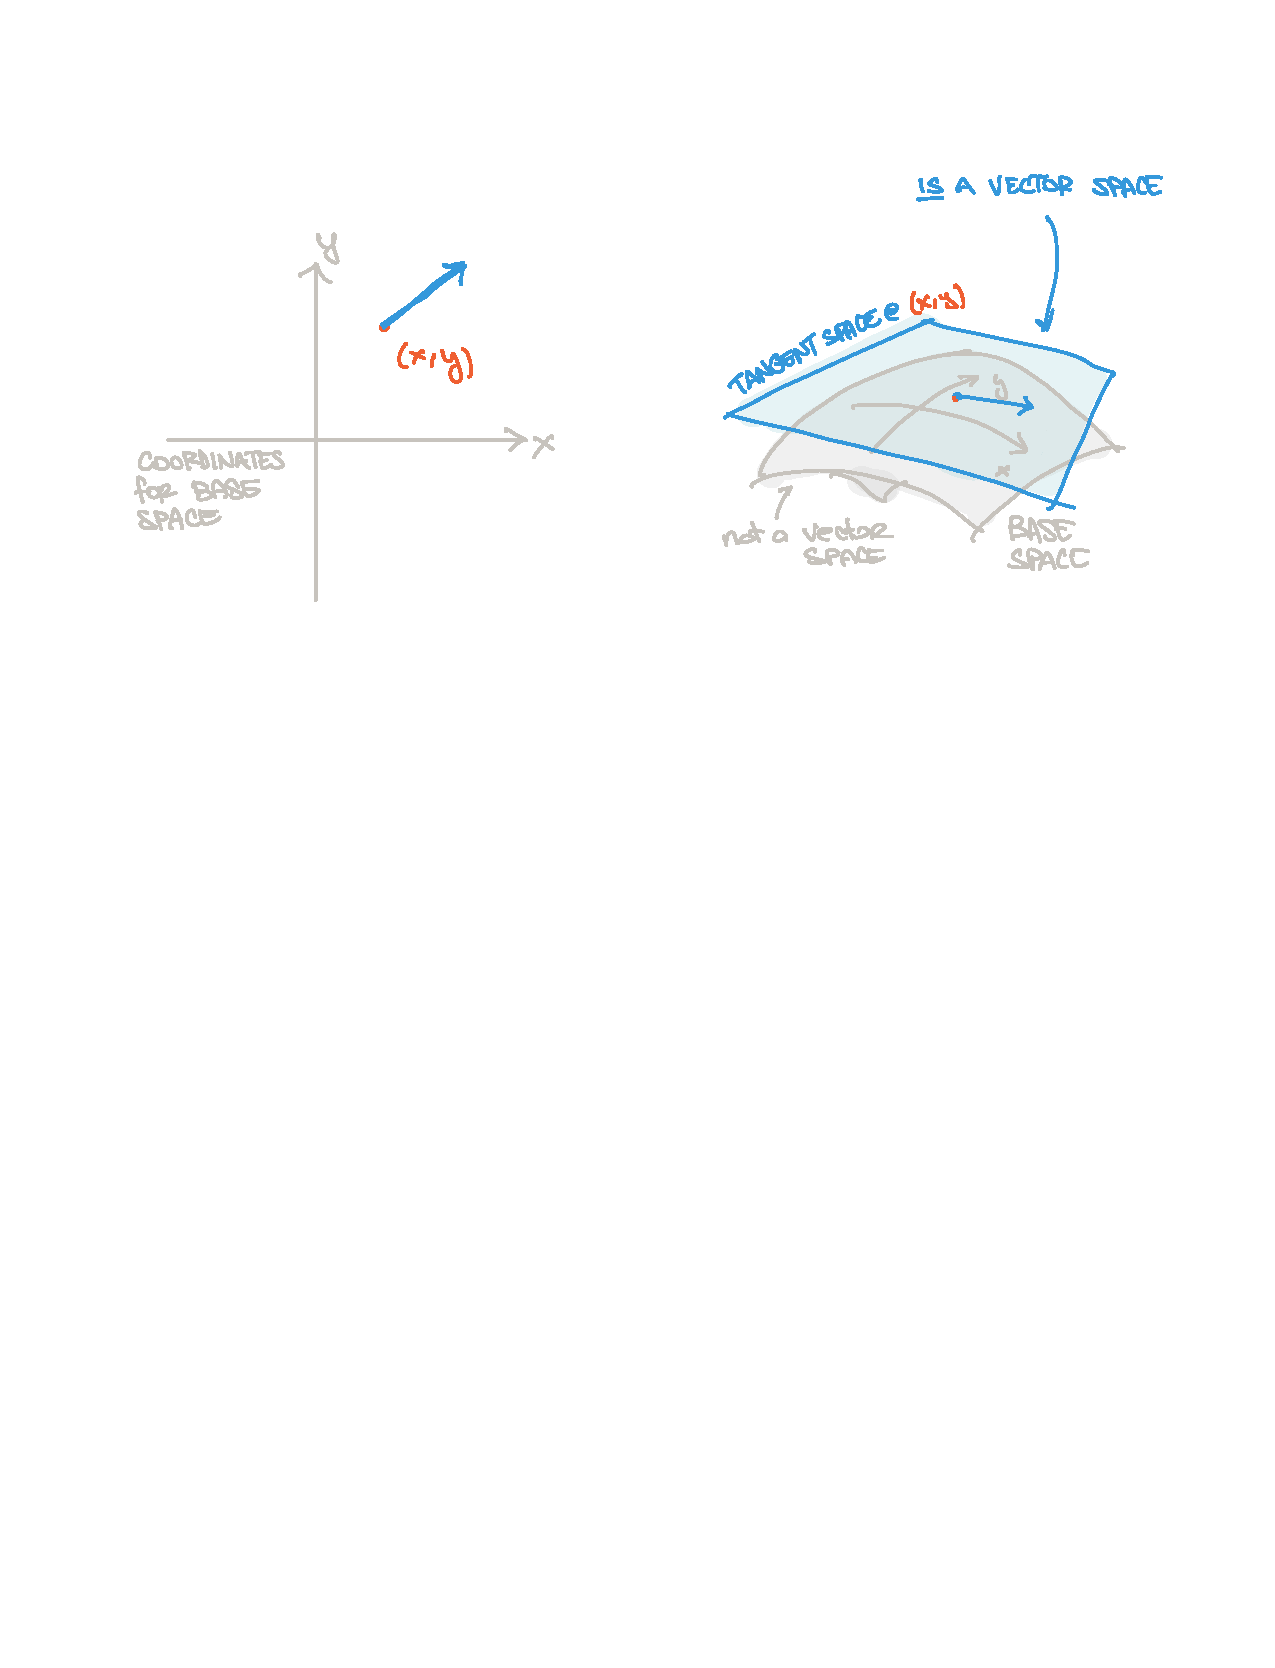
\includegraphics[width=\textwidth]{figures/base_space_tangent_space.pdf}
%     \captionsetup{font={scriptsize,sf}}
%     \caption{The base space is ``coordinate space.'' These are positions. Positions are not vectors and the base space is not a vector space. Positions depend on the coordinate system. At each position $(x,y)$, there is a vector space called the tangent space at $(x,y)$. This \emph{is} a vector space and the vectors can be thought of as possible velocities of a particle at $(x,y)$. In the picture on the right hand side we have `peeled' the base space away from the tangent space to make it clear that they are different, even though they both look like sheets of paper. There is no assumed curvature in the base space. There is a different tangent space for each position. The combination of the infinite number of tangent spaces over the base space is known as a tangent space bundle.}
%     \label{fig:tangent:space:polar}
% \end{marginfigure}

\begin{figure}[tb]
    \centering
    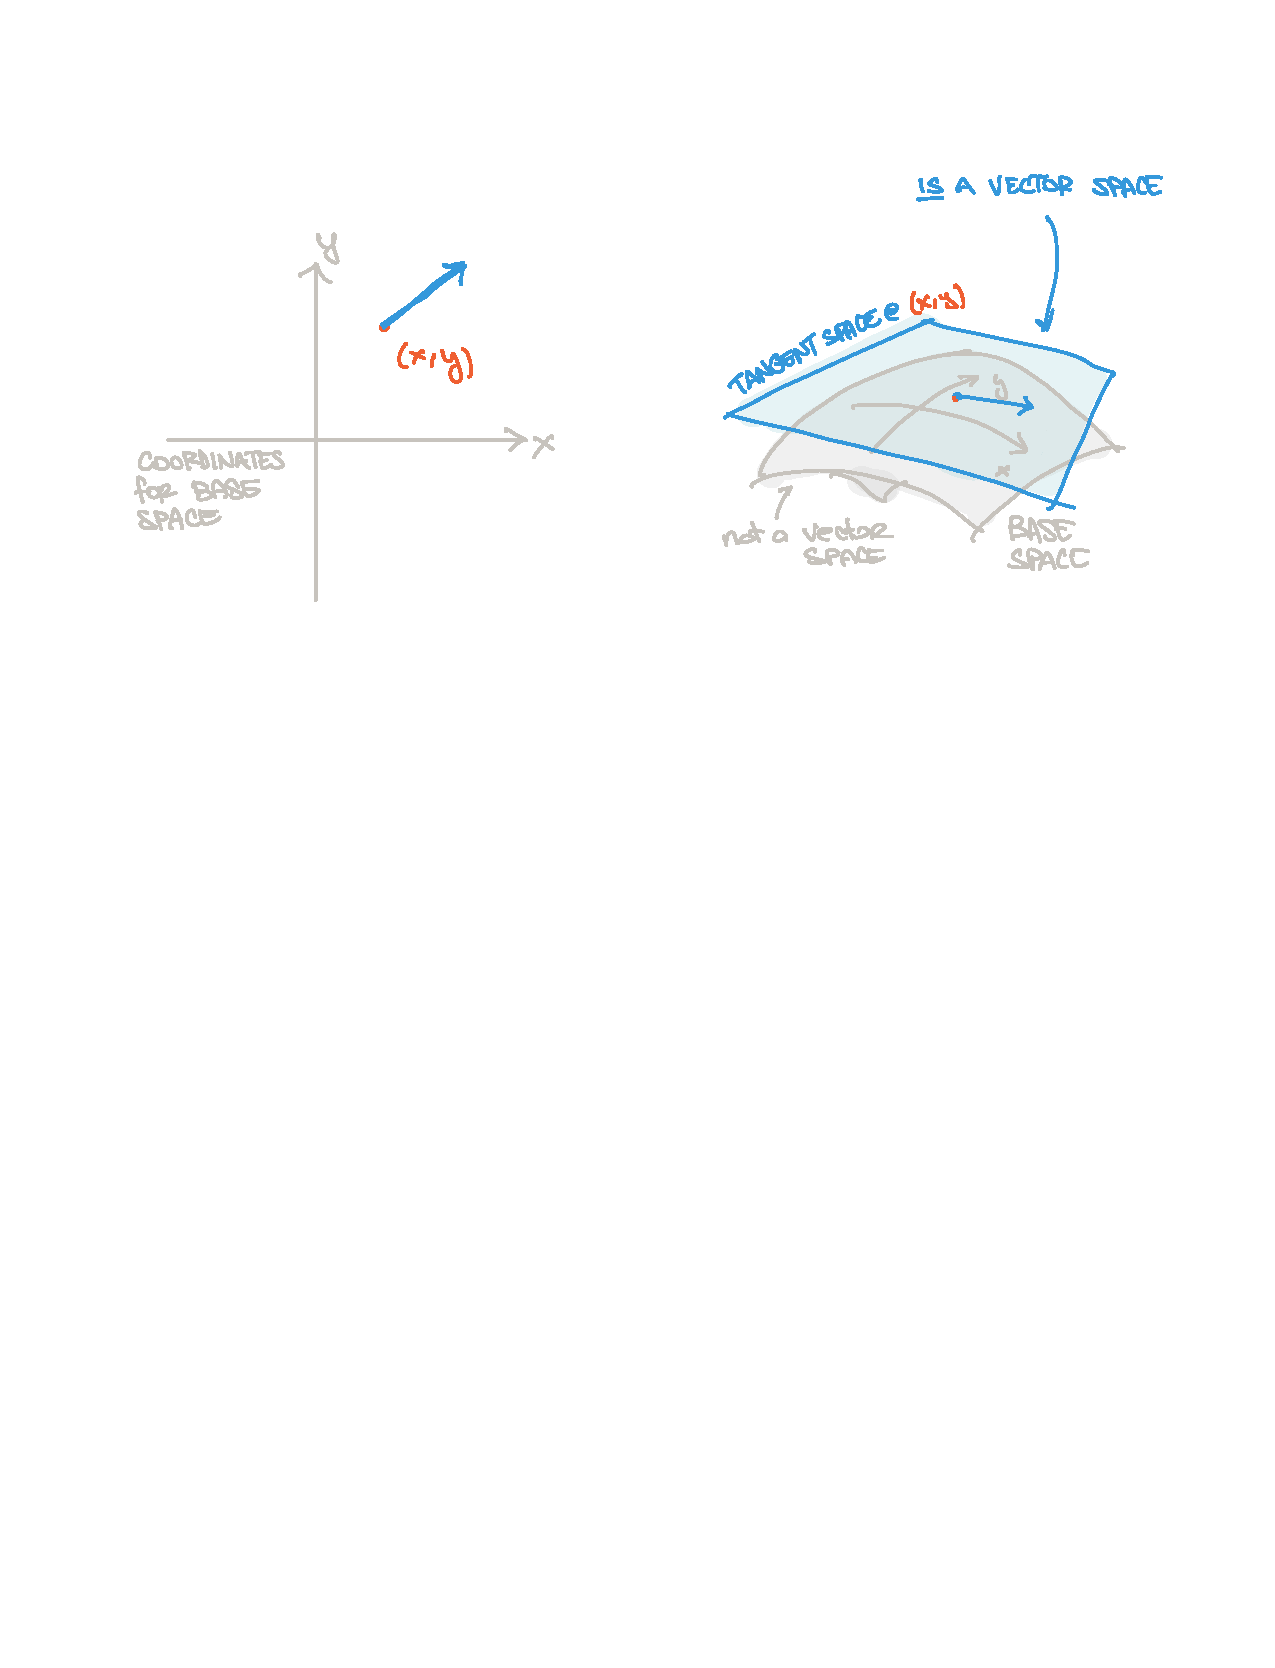
\includegraphics[width=.7\textwidth]{figures/base_space_tangent_space.pdf}
    \caption{The base space is ``coordinate space.'' These are positions. Positions are not vectors and the base space is not a vector space. Positions depend on the coordinate system. At each position $(x,y)$, there is a vector space called the tangent space at $(x,y)$. This \emph{is} a vector space and the vectors can be thought of as possible velocities of a particle at $(x,y)$. In the picture on the right hand side we have `peeled' the base space away from the tangent space to make it clear that they are different, even though they both look like sheets of paper. There is no assumed curvature in the base space. There is a different tangent space for each position. The combination of the infinite number of tangent spaces over the base space is known as a tangent space bundle.}
    \label{fig:tangent:space:polar}
\end{figure}

The tangent bundle picture of vectors also explains the following maxim that I have repeated over and over:
\begin{quote}
\emph{There is no such thing as a position vector.}
\end{quote}
Vectors live in a tangent space $\textnormal{T}_pM$. On a tangent space there is a natural meaning of the zero vector: it is the case of zero velocity. However, \emph{positions} live on the manifold, $M$. There is \emph{no} natural meaning of a `zero' position: that is simply an arbitrary choice of the origin of coordinates. Because the origin has no significance, there is also no natural meaning for taking a linear combination of positions.\sidenote{On the other hand, \emph{differences} of positions \emph{can} have physical meanings since they do not depend on an arbitrary origin.}

\begin{example}
In a vector space, the zero vector is special because it is the additive identity. Any vector plus the zero vector is well defined: it returns the vector itself,
\begin{align}
    \vec{v} + \vec{0} = \vec{v} \ .
\end{align}
If I define a coordinate system for space, the zero point of that coordinate system means nothing. There is no meaningful sense in which you can \emph{add} that position to another position, let alone for it to be understood to be the additive identity. 

However, differences of positions are meaningful vectors. The zero vector is when two points are coincident. Adding the zero vector does not change the separation between two points. 
\end{example}


\section{Taylor Expansion, yet again}

Curved manifolds are, unsurprisingly, much more difficult than flat ones. One way of seeing the preponderance of vector spaces in physics is that these vectors are the leading terms in the evolution of a system whose trajectory on a manifold is $\gamma(t)$. That we write the velocity vector as $\dot\gamma(t)$ shows a significant relationship between derivatives and vector spaces. 

Suppose you have some function $f(p)$ that takes points on the manifold $p\in M$ and returns a number. For example, $f(p)$ may be the temperature at the point $p$ on the Earth. Given a trajectory $\gamma(t)$ on the Earth, one may ask that at a given time $t$ and point $p=\gamma(t)$, what is the instantaneous rate of change of the temperature? Let us write $\gamma^i(t)$ to mean the $i^\textnormal{th}$ coordinate of $\gamma(t)$.\sidenote{Note that $\gamma^i(t)$ is not the component of a vector. It is a component of a position, and positions are not vectors.}
% 
With respect to the ambient three dimensional space, this rate of change is
\begin{align}
    \dot f(\gamma(t)) = \frac{\D{f(\gamma(t))}}{\D{t}} = 
    \frac{\partial f}{\partial \gamma^i}
    \frac{\D{\gamma^i(t)}}{\D{t}}
    % \frac{\partial f(t)}{\partial x^i}  \frac{\partial x^i}{\partial t} \bas{e}_i \ ,
\end{align}
Here we recognize that $v^i= \D{\gamma^i(t)}/\D{t}$ \emph{is} the component of a vector. This is because \emph{differences} of positions are vectors, even if positions themselves are not. Thus we may write
\begin{align}
    \dot f(\gamma(t)) %= \frac{\D{f(\gamma(t))}}{\D{t}} = 
    \frac{\D{\gamma^i(t)}}{\D{t}}
    \frac{\partial}{\partial \gamma^i}
    f(\gamma(t))
    =
    v^i
    \frac{\partial}{\partial \gamma^i}
    f(\gamma(t)) \ .
    % \frac{\partial f(t)}{\partial x^i}  \frac{\partial x^i}{\partial t} \bas{e}_i \ ,
\end{align}
We recognize that\sidenote{I use the notation $\partial_x = \frac{\partial}{\partial x}$.} $v^i \partial_{\gamma^i}$ looks like a velocity vector with a basis given by the partial derivatives. Indeed, we often write that this allows us to treat the partial derivatives with respect to the manifold $M$ are a \emph{basis} for the tangent space.\sidenote{In this case the sphere is embedded in the three dimensional space, so there are possible three basis vectors. However, each tangent space is two dimensional. This is consistent because $v^i= \D{\gamma^i(t)}/\D{t} = 0$ in the direction that is perpendicular to the surface. Thus one linear combination of partial derivatives always has a zero coefficient.} This idea of a vector as a linear combination of partial derivatives is quite helpful, albeit completely unusual the first time you see it. One can imagine that this sort if picture shows up all the time when dealing with flows.



\section{Microphysics lives in the tangent plane}

We present this picture as if you already know what the trajectory $\gamma(t)$ is. In physics, we often try to solve the opposite problem.  If you know the properties of a trajectory at some point $p=\gamma(0)$, can you \emph{integrate} the equations of motion to determine the trajectory at future times?\sidenote{The question of integrability of a vector field over a manifold is an open one in many important physical scenarios. Look up the phrase `integrable system.'}

A bit more philosophically: the laws of physics are defined microscopically. They relate the dynamics of the system at one point to the dynamics at nearby points. This is why our theories are all written with differential operators. Taking the picture that the tangent planes are approximations for moving along the manifold, everything that we call \emph{physics}\sidenote{Notably, equations of motion and the underlying structures from which they are derived.} is defined on how these tangent planes relate to each other. In this way, we can measure things like arclength on a trajectory by using the \emph{metric} (see Chapter~\ref{ch:metric:spaces}) and summing together the infinitesimal lengths of tangent vectors along the trajectory. The components of the metric are a \emph{field}\index{field} defined on the manifold, $g_{ij}(x)$. This means that the `rulers' we use to measure distance are warped if space is curved.\sidenote{The requirement that the connection between tangent planes may be metric compatible is one about the $x$-dependence of the components of the metric.} In general relativity, gravity is encoded in the metric. 

\section{Diffeomorphisms}

Often the tensors on the tangent bundle are defined with respect to the coordinates of the base space, $x$. As you saw in the previous sections, these can show up as partial derivatives with respect to these coordinates, which are a natural\sidenote{Natural, if somewhat unexpected.} basis for the tangent planes. The way we choose to place coordinates on a manifold, however, is not a property of the manifold: it is simply a choice that we make. Thus all these bundles must not depend on whether we choose one reasonable set of coordinates versus another. This is called \emph{diffeomorphism invariance}. When we change coordinates on $M$, say from $x\to y,$ the quantities on the tangent planes also change coordinates. Because those quantities are written with respect to partial derivatives, the transformations look like\sidenote{Note that an upper index in the denominator contracts like a lower index. It is one of the convenient quirks of the summation convention. Convince yourself that this makes sense.}
\begin{align}
    \frac{\partial}{\partial x^i} \to 
    \frac{\partial y^j}{\partial x^i} 
    \frac{\partial}{\partial y^j}  \ .
\end{align}
Thus in relativity you will often see change of coordinates written as ${\partial y^j}/{\partial x^i}$. On a given tangent plane, these play the role of generalized rotation matrices.


\begin{bigidea}
Through this part of the course, the rules for how a tensor transforms in Section~\ref{sec:transformation:under:symmetries} are true for \emph{any} transformation, including diffeomorphisms if one is on a bundle. In that section and in most of this course, we focus only on the case when these transformations are rotations (or their generalizations, isometries). The reason for this is that in Chapter~\ref{ch:metric:spaces} we introduce the inner product, which defines a special class of transformations---rotations (isometries)---which are the main focus of our course. However, an object with indices is a tensor if it transforms tensorially under \emph{any} transformation, including diffeomorphisms. 
\end{bigidea}
The above \bigidearef{} comes up again in Section~\ref{sec:Levi:Civita:Tensor:vs:Symbol} when we look at an object called the Levi-Civita tensor.



\section{Bundles of Fun}

The rich structure of vector spaces and dual vector spaces become richer on a bundle. Just as there is a tangent bundle $\textnormal{T}_pM$, there is also a co-tangent bundle $\textnormal{T}^*_pM$ where dual vectors live. There are other types of fields that live on the manifold and tell us about how to move between the spaces that live `over' a point $p$. If you are mathematically inclined, a good way to start thinking about bundles is to think about the M\"obius strip as the prototype of a bundle with non-trivial \emph{global} properties, see e.g.\ Collinucci and Wijns\autocite{Collinucci:2006hx}.

For more introductory references on how this structure appears in ordinary mechanics, I refer to two neat graduate-level textbooks in Fig.~\ref{fig:figure:mathematical:physics:books}. If you want to deeply appreciate the differences between the Lagrangian and Hamiltonian formulation of mechanics, you may enjoy these books. For example, momenta are part of the cotangent bundle while velocities are part of the tangent bundle. 
\begin{marginfigure}%[th]
    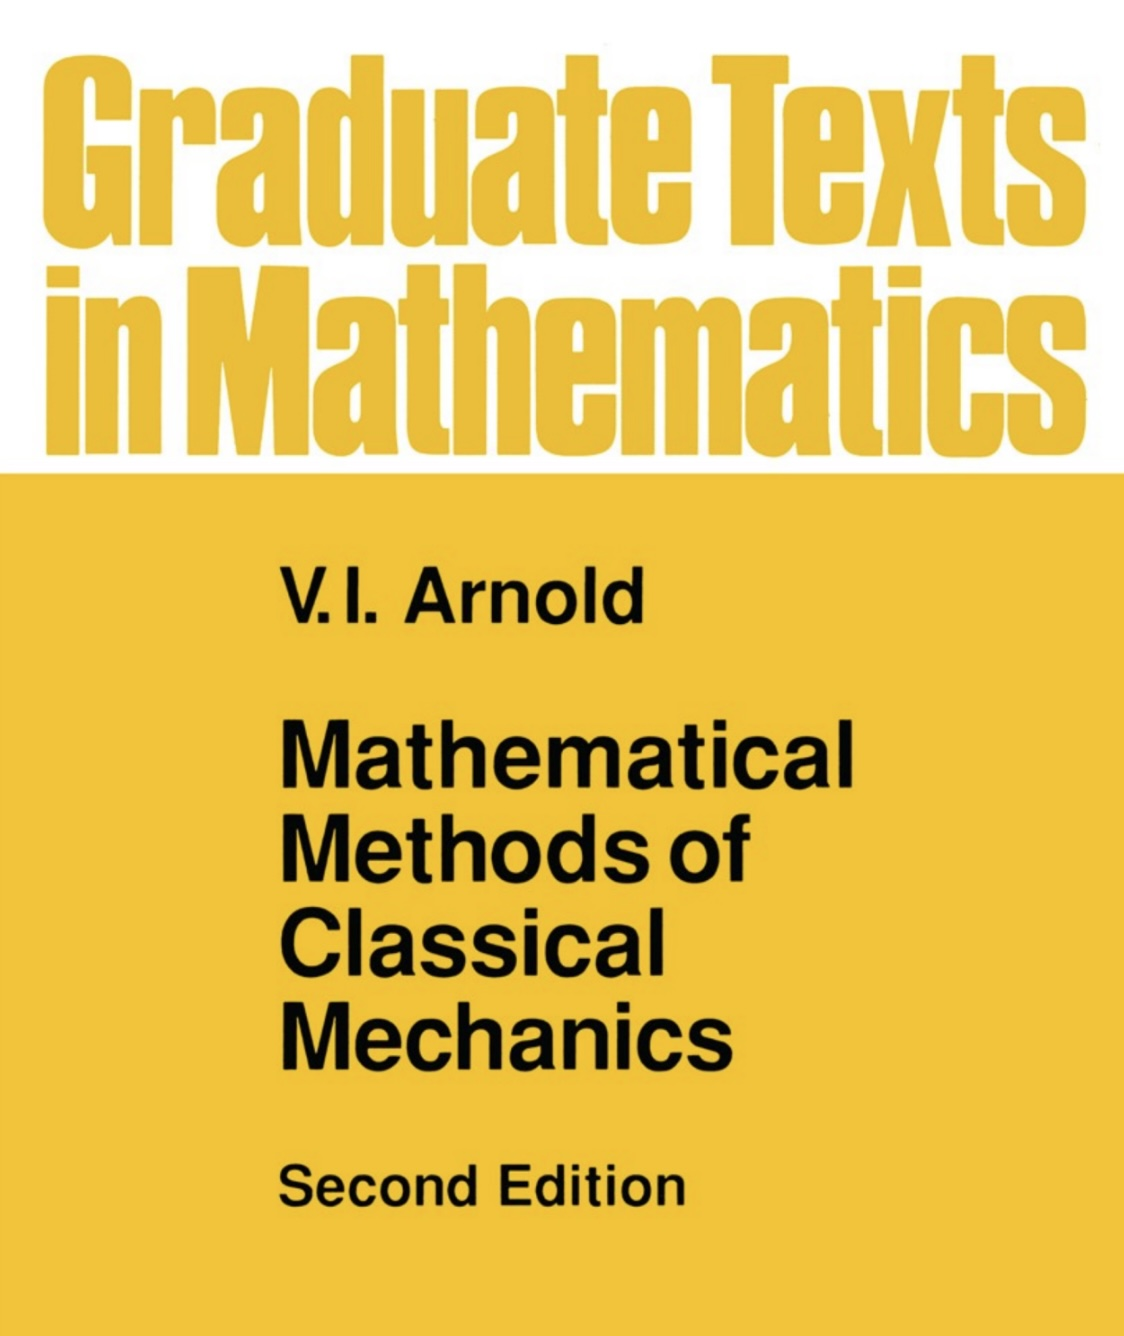
\includegraphics[width=.6\textwidth]{figures/Arnoldbook.jpg}\\
    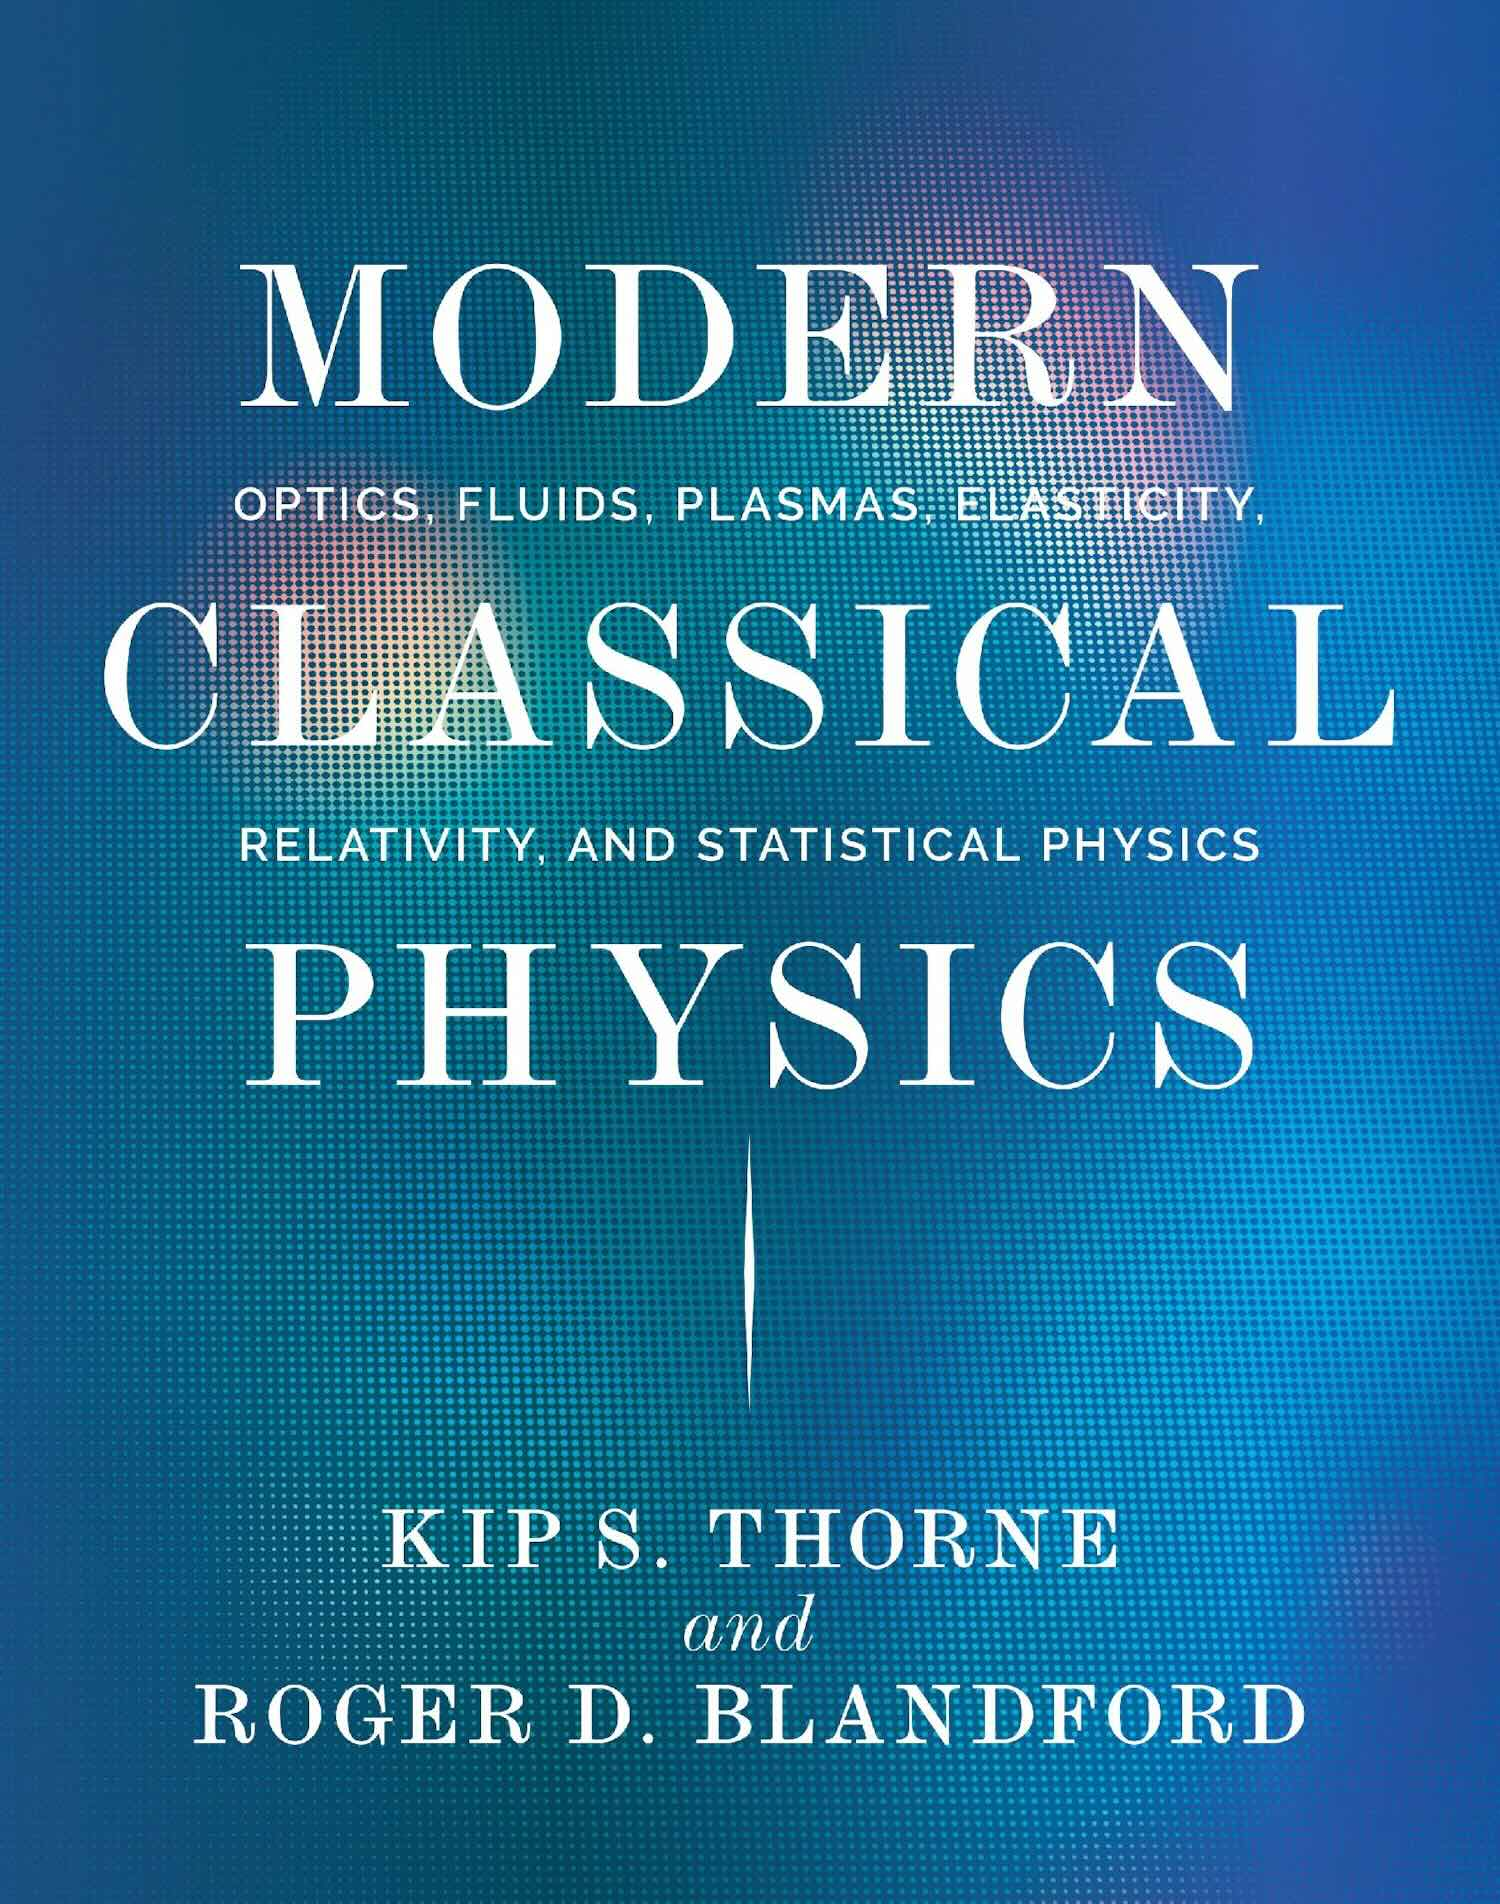
\includegraphics[width=.6\textwidth]{figures/MCP_Thorne.jpg}
    \captionsetup{font={scriptsize,sf}}
    \caption{Two excellent references to go over some physics that you know (mechanics) in the language of differential geometry.}
    \label{fig:figure:mathematical:physics:books}
\end{marginfigure}

The fundamental forces in subatomic physics are part of a structure called a \textbf{gauge theory }\index{gauge theory} which is mathematically a bundle over spacetime. Unlike tangent or co-tangent bundles, the vector space living `on top' of each point $p$ needn't strictly be a tangent space. These vector spaces are called fibers. In electromagnetism, the fiber is the choice of gauge.\sidenote{Recall from electrodynamics that the vector and scalar potentials can be shifted by the derivative of a function of spacetime. This is called gauge symmetry.} This gauge is a redundancy in how we describe a system. The redundancy is necessary to maintain manifest spacetime symmetries in the theory. The \emph{connection} on such a structure is called the gauge potential---this is precisely the vector and scalar potentials. In the quantum version of electrodynamics, this gauge potential is the quantum field associated with the photon. Analogously, there is a fiber bundle picture for fundamental forces---such a picture exists for gravity as well, though I have never had the occasion to make use of it. 
